%TODO:
    %- normal data structures (manual memory management)
    %- there is no other evaluation (experimental or otherwise) provided.

%\documentclass[preprint]{sigproc}
\documentclass[preprint]{sigplanconf}

% The following \documentclass options may be useful:
%
% 10pt          To set in 10-point type instead of 9-point.
% 11pt          To set in 11-point type instead of 9-point.
% authoryear    To obtain author/year citation style instead of numeric.

\setlength{\textfloatsep}{5pt}

\usepackage{flushend}
\usepackage{graphicx}
\usepackage{verbatim}
\usepackage{url}
\usepackage{alltt}
\renewcommand{\ttdefault}{txtt}

\usepackage{amsmath}
\usepackage{dsfont}
\usepackage{mathtools}
\everymath{\displaystyle}
\usepackage{xspace}

\usepackage[bottom]{footmisc}

\newcommand{\CEU}{\textsc{C\'{e}u}\xspace}
\newcommand{\code}[1] {{\small{\texttt{#1}}}}
\newcommand{\DOFIN}{\code{do-finally}\xspace}
\newcommand{\FIN}{\code{finally}\xspace}

\newcommand{\ST}{\1\xrightarrow[~n~]{}\1}
\newcommand{\BT}{\xRightarrow[(i,E)]{}}
\newcommand{\LL}{\langle}
\newcommand{\RR}{\rangle}
\newcommand{\DS}{\displaystyle}
\newcommand{\rr}[1] {{\textbf{\scriptsize{#1}}}}


\newcommand{\1}{\;}
\newcommand{\2}{\;\;}
\newcommand{\3}{\;\;\;}
\newcommand{\5}{\;\;\;\;\;}
\newcommand{\ten}{\5\5}
\newcommand{\twenty}{\ten\ten}
\newcommand{\URL}{\small\url}

\newenvironment{itemize*}%
  {\begin{itemize}%
    \setlength{\itemsep}{0pt}%
    \setlength{\parskip}{0pt}}%
  {\end{itemize}}

\usepackage{enumitem}
\setlist{nolistsep}

\usepackage{color}
\definecolor{light}{gray}{0.87}
\definecolor{dark}{gray}{0.30}
%\definecolor{light}{rgb}{.90,.90,.90}
\definecolor{darkgreen}{rgb}{0,.50,0}
\definecolor{darkblue}{rgb}{0,0,.50}
\definecolor{darkred}{rgb}{.50,0,0}
\definecolor{darkpur}{rgb}{.50,0,.50}

\usepackage{listings}
%\usepackage{textcomp}
\lstset{
%columns=fullflexible,
%basicstyle=\ttfamily,
escapeinside={||},
mathescape=true,
    language=C, % choose the language of the code
    basicstyle=\fontfamily{pcr}\selectfont\scriptsize\color{black},
    keywordstyle=\color{black}\bfseries, % style for keywords
    numbers=none, % where to put the line-numbers
    numberstyle=\tiny, % the size of the fonts that are used for the line-numbers
    backgroundcolor=\color{light},
    showspaces=false, % show spaces adding particular underscores
    showstringspaces=false, % underline spaces within strings
    showtabs=false, % show tabs within strings adding particular underscores
    %frame=single, % adds a frame around the code
    tabsize=2, % sets default tabsize to 2 spaces
    %rulesepcolor=\color{gray}
    captionpos=b, % sets the caption-position to bottom
    breaklines=false, % sets automatic line breaking
    %breakatwhitespace=false,
    numbersep=2em,
    emph={par,or,hor,do,end,loop,await,emit,input,event,call,with,command,%
          var,and,then,else,C,return,pure,deterministic,nohold,finalize,%
          class, every, FOREVER, this, spawn, in, pool, watching, until, 
          interface, each, abort, when, signal, PROC, CHAN, SIGNAL, PAR, not,
          bool},
    emphstyle={\bfseries},
    commentstyle=\color{dark}\scriptsize,
    %xleftmargin=20pt,
    %xrightmargin=20pt,
    framesep=20pt,
    %upquote=true,
    %aboveskip={1.5\baselineskip},
}

\begin{document}
\sloppy

\special{papersize=8.5in,11in}
\setlength{\pdfpageheight}{\paperheight}
\setlength{\pdfpagewidth}{\paperwidth}

\conferenceinfo{CONF 'yy}{Month d--d, 20yy, City, ST, Country} 
\copyrightyear{20yy} 
\copyrightdata{978-1-nnnn-nnnn-n/yy/mm} 
\doi{nnnnnnn.nnnnnnn}

\title {
    %Imperative and Synchronous Abstractions for Reactive Applications
    %Structured Programming with Reactive Abstractions
    Structured Synchronous Reactive Programming with C\'eu
}
%\subtitle{Accepted paper in REM'13 (preprint version)}

%\authorinfo{Francisco Sant'Anna}
           %{Departamento de Inform\'atica --- PUC-Rio, Brazil}
           %{fsantanna@inf.puc-rio.br}
%\authorinfo{Roberto Ierusalimschy}
           %{Departamento de Inform\'atica --- PUC-Rio, Brazil}
           %{roberto@inf.puc-rio.br}
%\authorinfo{Noemi Rodriguez}
           %{Departamento de Inform\'atica --- PUC-Rio, Brazil}
           %{noemi@inf.puc-rio.br}

\authorinfo{}{}{}

\maketitle

\begin{abstract}
Structured synchronous reactive programming (SSRP) augments classical 
structured programming (SP) with continuous interaction with the environment.
%
We advocate SSRP as viable in multiple domains of reactive applications and 
propose a new abstraction mechanism for the synchronous language \CEU:
%
\emph{Organisms} extend objects with an execution body that composes multiple 
lines of execution to react to the environment independently.
%
Compositions bring structured reasoning to concurrency and can better describe 
state machines typical of reactive applications.
%
Organisms are subject to lexical scope and automatic memory management similar 
to stack-based allocation for local variables in SP.
We show that this model does not require garbage collection or a \code{free} 
primitive in the language, eliminating memory leaks by design.
\end{abstract}

%\category{CR-number}{subcategory}{third-level}
%\category{D.3.1}{Programming Languages}{Formal Definitions and Theory}
%\category{D.3}{Programming Languages}{General}
\category{D.3.3}{Programming Languages}{Language Constructs and Features}

\terms{Design, Languages}

\keywords{Concurrency, Determinism, Esterel, Imperative, Structured 
Programming, Synchronous, Reactivity}

\section{Introduction}
\label{sec.intro}

Reactive applications interact continuously and in real time with external 
stimuli from the environment~\cite{statecharts.reactive,rp.synchronous}.
They represent a wide range of software areas and platforms: from games in 
powerful desktops and ``apps'' in capable smart phones, to the emerging 
internet of things in constrained embedded systems.

Research on special-purpose reactive languages dates back to the early 80's, 
with the co-development of two complementary 
styles~\cite{rp.twelve,rp.hypothesis}:
%
The imperative style of Esterel~\cite{esterel.ieee91} organizes programs with 
structured control flow primitives, such as sequences, repetitions, and 
parallelism.
%
The dataflow style of Lustre~\cite{lustre.ieee91} represents programs as graphs 
of values, in which a change to a node updates its dependencies automatically.
%
Both styles rely on the \emph{synchronous execution hypothesis} which states 
that the input and corresponded output in reactions to the environment are 
simultaneous because, in this context, internal computations should run 
infinitely faster than the rate of events~\cite{rp.hypothesis}.

In recent years, Functional Reactive Programming (FRP)~\cite{frp.principles} 
has modernized the dataflow style, inspiring a number of languages and 
libraries, such as Flapjax~\cite{frp.flapjax}, Rx (from Microsoft), React (from 
Facebook), and Elm~\cite{frp.elm}.
%
In contrast, the imperative style of Esterel is confined to the domain of 
real-time embedded control systems.
% such as flight control on avionics and anti-collision equipment on automobiles.
%
As a matter of fact, imperative reactivity is now often associated to the 
\emph{observer pattern}, typical in object-oriented systems, due to its heavy
reliance on side effects~\cite{rp.deprecating,rp.rescala,gamepatterns}.
%
However, short-lived callbacks (i.e., the observers) eliminate any vestige of 
structured programming, such as support for long-lasting loops and automatic 
variables~\cite{sync_async.cooperative}, which are elementary capabilities of 
imperative languages.
%
In this sense, callbacks actually disrupt imperative reactivity, becoming ``our 
generation's \code{goto}''.%
\footnote{``Callbacks as our Generations' Go To Statement'':
\url{http://tirania.org/blog/archive/2013/Aug-15.html}}%
\footnote{``Escape from Callback Hell'':
\url{http://elm-lang.org/learn/Escape-from-Callback-Hell.elm}}

We believe that all domains of reactive applications can benefit from the 
imperative style of Esterel, which we now refer to as \emph{Structured 
Synchronous Reactive Programming (SSRP)}.
%
SSRP extends the classical hierarchical control constructs of \emph{Structured 
Programming (SP)} (i.e., concatenation, selection, and 
repetition~\cite{dij.notes}) to support continuous interaction with the 
environment.
%
In contrast with FRP, SSRP retains structured and sequential reasoning of 
concurrent programs, bringing the historical dichotomy between functional and 
imperative languages also to the reactive domain.
%
However, the original rigorous semantics of Esterel, which focuses on static 
safety guarantees, is not suitable for other reactive application domains, such 
as GUIs, games, and distributed systems.
%
For instance, the lack of abstractions with dynamic lifetime makes it difficult 
to deal with virtual resources such as graphical widgets, game units, and 
network sessions.

In practical terms, SSRP provides three extensions to SP:
an ``\code{await <event>}'' statement that suspends a line of execution until 
the referred event occurs, keeping all context alive;
parallel constructs to compose multiple lines of execution and make them 
concurrent;
and an orthogonal mechanism to abort parallel compositions.
%
The \code{await} statement represents the imperative-reactive nature of SSRP, 
recovering sequential execution lost with the observer pattern.
%
Parallel compositions%
\footnote{
In this work, the term \emph{parallel composition} does not imply many-core 
parallel execution.
}
allow for multiple \code{await} statements to coexist, which is necessary to 
handle concurrent events, common in reactive applications.
%
Orthogonal abortion is the ability to abort an activity from outside it, 
without affecting the overall consistency of the program (e.g., properly 
releasing global resources).

In this work, we extend the Esterel-based language \CEU~\cite{ceu.sensys13} 
with a new abstraction mechanism, the \emph{organisms}, that encapsulate 
parallel compositions with an object-like interface.
% that other parts of the program can manipulate.
%
In brief, organisms are to SSRP like procedures are to SP, i.e., one can 
abstract a portion of code with a name and manipulate (call) that name from 
multiple places.
%
Unlike procedure calls in multi-threaded applications, organisms have 
deterministic behavior and do not require explicit synchronization.
%
Unlike Simula objects~\cite{simula}, organisms react independently to the 
environment and do not depend on cooperation, i.e., once instantiated they 
become alive and reactive (hence the name organisms).
%
%
Furthermore, organisms are subject to lexical scope and automatic memory 
management for both static and dynamic instances, not relying on heap 
allocation at all.
%(behaving much like local variables in SP).
%
%Organisms retain control and can describe, in a self-contained and structured 
%style, continuous control behavior, such as independent state machines for 
%network packets, or XXX in games.

%TODO: o que ganha com orgs

\begin{comment}
There are, however, additional challenges that apply to organisms:
%
\begin{itemize}
\item Organisms are themselves alive, acting as subprograms with continuous 
data and control state.
\item Organisms are part of a concurrent program that can manipulate and affect 
their data and execution state.
\item Organisms can be dynamically allocated, requiring a memory management 
model that must also apply to embedded systems.
\end{itemize}
\end{comment}

The rest of the paper is organized as follows:
%Section~\ref{sec.models} justifies the synchronous concurrency model as better 
%choice for SSRP.
Section~\ref{sec.ceu} presents SSRP through \CEU, with its underlying 
synchronous concurrency model and parallel compositions.
Section~\ref{sec.orgs} describes the organisms abstraction with static and 
dynamic instantiation, lexical scope, and automatic memory management.
Section~\ref{sec.apps} demonstrates two complete applications developed 
entirely with SSRP in \CEU: a network protocol for sensor networks and a video 
game for tablets.
Section~\ref{sec.related} discusses related work.
Section~\ref{sec.conclusion} concludes the paper.

\section{SSRP with C\'eu}
\label{sec.ceu}

\CEU is a concurrent language in which the lines of execution, known as 
\emph{trails}, react all together continuously and in synchronous steps to 
external stimuli.
%
%Figure~\ref{lst.syntax} shows a compact reference of \CEU.
%
The introductory example in Figure~\ref{lst.intro} defines an input event 
\code{RESET} (line 1), a shared variable \code{v} (line 2), and starts two 
trails with the \code{par} construct (lines 3-14): the first (lines 4-8) 
increments variable \code{v} on every second and prints its value on screen; 
the second (lines 10-13) resets \code{v} on every external request to 
\code{RESET}.
%
%The input event \code{RESET} (line 1) represents the interface of the program 
%with external requests.
%The loop in the first trail (lines 4-8) continuously waits for 1 second, 
%increments variable \code{v}, and prints its current value.
%The loop in the second trail (lines 10-13) resets \code{v} on every occurrence 
%of \code{RESET}.
%
Programs in \CEU can access \emph{C} libraries of the underlying platform 
directly by prefixing symbols with an underscore (e.g., \code{\_printf(<...>)}, 
in line 7).

\begin{comment}
\begin{figure}%[t]
\begin{lstlisting}%[backgroundcolor=\color{white}]

// DECLARATIONS
input <type> <id>;        // external event
event <type> <id>;        // internal event
var   <type> <id>;        // variable

// EVENT HANDLING
await <id>;               // awaits event
emit  <id> => <exp>;      // emits  event

// COMPOUND STATEMENTS
<...> ; <...> ;           // sequence
if <...> then <...>       // conditional
         else <...> end
loop do <...> end         // repetition
    break                 //   (escape repetition)

// PARALLEL COMPOSITIONS
par/and do <...>          // rejoins on both sides
      with <...> end
par/or do  <...>          // rejoins on any side
      with <...> end
par do <...>              // never rejoins
  with <...> end

// C INTEGRATION
_f();                     // C call (prefix `_')
finalize <...>            // finalization
    with <...> end

// ORGANISMS
class <T> with            // class definition
    <interface>
do
    <body>
end
var <T> <id> with         // static instantiation
    <constructor>
end;
spawn <T> with            // dynamic instantiation
    <constructor>
end;
\end{lstlisting}
%\rule{8.5cm}{0.37pt}
\caption{ Syntax of \CEU.
\label{lst.syntax}
}
\end{figure}
\end{comment}

%%%%%%%%%%%%%%%%%%%%%%%%%%%%%%%%%%%%%%%%%%%%%%%%%%%%%%%%%%%%%%%%%%%%%%%%%%%%%%%
\subsection{Synchronous concurrency}
\label{sec.ceu.sync}
%%%%%%%%%%%%%%%%%%%%%%%%%%%%%%%%%%%%%%%%%%%%%%%%%%%%%%%%%%%%%%%%%%%%%%%%%%%%%%%

In \CEU, a program reacts to an occurring event completely before handling the 
next.
%
A reaction represents a logical instant in which all trails awaiting the 
occurring event awake and execute, one after the other, until they await again 
or terminate.
%
During a reaction, the environment is invariant and does not interrupt the 
running trails%
\footnote{
The actual implementation enqueues incoming input events to process them in 
further reactions.
}.
If multiple trails react to the same event, the scheduler employs lexical order 
to preserve determinism, i.e., the trail that appears first in the source code 
executes first.
% TODO: For this reason, await vs exec in parallel
%
To avoid infinite execution for reactions, \CEU ensures that all loops contain 
\code{await} statements~\cite{ceu.sensys13}.

% TODO: rules? (slides da aula)

As a consequence of synchronous execution, all consecutive operations to shared 
variable \code{v} in Figure~\ref{lst.intro} are atomic (until reaching the next 
\code{await}) because reactions to events \code{1s} and \code{RESET} can never 
interrupt each other.
%
In contrast, in asynchronous models with nondeterministic scheduling, the 
occurrence of \code{RESET} could preempt the first trail during an increment to 
\code{v} (line 6) and reset it (line 12) before printing it (line 7), 
characterizing a race condition on the variable.
%
The example illustrates the (arguably simpler) reasoning about concurrency 
under the synchronous execution model.

\begin{figure}%[t]
\begin{lstlisting}[numbers=left,xleftmargin=3em]
input void RESET;   // declares an external event
var int v = 0;      // variable shared by the trails
par do
    loop do         // 1st trail
        await 1s;
        v = v + 1;
        _printf("v = %d\n", v);
    end
with
    loop do         // 2nd trail
        await RESET;
        v = 0;
    end
end
\end{lstlisting}
\caption{ Introductory example in \CEU.
\label{lst.intro}
}
\end{figure}

%%%%%%%%%%%%%%%%%%%%%%%%%%%%%%%%%%%%%%%%%%%%%%%%%%%%%%%%%%%%%%%%%%%%%%%%%%%%%%%

The synchronous model also empowers SP with an orthogonal abortion construct 
that simplifies the composition of activities%
\footnote{We use the term activity to generically refer to a language's unit of 
execution (e.g., \emph{thread}, \emph{actor}, \emph{trail}, etc.).}.
%
%Orthogonal abortion is the ability to abort an activity from outside it, 
%without affecting the overall consistency of the program (e.g., properly 
%releasing global resources).
%
The code that follows shows the \code{par/or} construct of \CEU which composes 
trails and rejoins when either of them terminates, properly aborting the other:

\begin{lstlisting}
par/or do
    <trail-1>
with
    <trail-2>
end
<subsequent-code>
\end{lstlisting}

%Each trail has a set of local variables and an execution body that lasts for 
%an arbitrary time.
%After the \code{par/or} rejoins, a new set of local variables goes alive, 
%reusing the space from the trails' locals which are now out of scope.

The \code{par/or} is regarded as orthogonal because the composed trails do not 
know when and how they are aborted (i.e., abortion is external to them).
%
This is possible in synchronous languages due to the accurate control of 
concurrent activities, i.e., in between every reaction, the whole system is 
idle and consistent~\cite{esterel.preemption}.
%
\CEU extends orthogonal abortion to also work with activities that use stateful 
resources from the environment (such as file and network handlers), as we 
discuss in Section~\ref{sec.ceu.par}.

%\begin{figure}%[t]
%\caption{ A \code{par/or} composes two concurrent trail and rejoins when one 
%terminates, aborting the other.
%\label{lst.abortion}
%}
%\end{figure}

Abortion in asynchronous languages is challenging~\cite{esterel.preemption} 
because the activity to be aborted might be on a inconsistent state (e.g., 
holding pending messages or locks).
%
This way, the possible (unsatisfactory) semantics for a hypothetical 
\code{par/or} are:
either wait for the activity to be consistent before rejoining, making the 
program unresponsive to incoming events for an arbitrary time;
or rejoin immediately and let the activity complete in the background, which 
may cause race conditions with the subsequent code.
%
%which may confuse the programmer (which assumes both activities have 
%terminated), and also
%Immediate rejoin also implies heap-based allocation for locals (which is 
%discouraged in the context of embedded systems) because activities may coexist 
%with the subsequent code for some time.
%
In fact, asynchronous languages do not provide effective abortion:
\emph{Java}'s \code{Thread.stop} primitive has been 
deprecated~\cite{sync_async.threadsstop};
\emph{pthread}'s \code{pthread\_cancel} does not guarantee immediate 
cancellation~\cite{sync_async.pthreadsstop};
\emph{Erlang}'s \code{exit} either enqueues a terminating message (which may 
take time), or unconditionally terminates the process (regardless of its 
state)~\cite{sync_async.erlangstop};
and \emph{CSP} only supports a composition operator that \emph{``terminates 
when \textbf{all} of the combined processes terminate''}~\cite{async.csp}.
%
As an alternative, asynchronous activities typically agree on a common protocol 
to abort each other (e.g., through shared state variables or message passing), 
which increases coupling among them with implementation details that are not 
directly related to the problem specification.

%TODO: talvez falar em termos de controle e dados

%\CEU provides the presented \code{par/or} construct, which is equivalent to 
%Esterel's \code{trap} abortion construct.
%
%In Section~\ref{sec.orgs} we highlight the importance of abortion for the 
%organisms abstraction.

%%%%%%%%%%%%%%%%%%%%%%%%%%%%%%%%%%%%%%%%%%%%%%%%%%%%%%%%%%%%%%%%%%%%%%%%%%%%%%%

%\subsection{The case for synchrony}

\subsection{Parallel compositions}
\label{sec.ceu.par}

\begin{comment}
- besides standard structured (loops, conditionals, sequences)
- add compositions
- await, sequence, vars
- parallel, patterns, orthogonal
- finalize for C integration and keep orthogonality
    - no await inside it
- not really parallel (prev section)
\end{comment}

In terms of control structures, SSRP basically extends SP with parallel 
compositions, allowing applications to handle multiple events concurrently.
%
\CEU provides three parallel constructs that vary on how they rejoin:
a \code{par/and} rejoins when all trails in parallel terminate;
a \code{par/or} rejoins when any trail in parallel terminates;
a \code{par} never rejoins (even if all trails in parallel terminate).
%
The code chunks that follow compare the \code{par/and} and \code{par/or} 
compositions side by side:

\begin{minipage}[t]{0.40\linewidth}
\begin{lstlisting}
loop do
    par/and do
        <...>
    with
        await 1s;
    end
end
\end{lstlisting}
\end{minipage}
%
\begin{minipage}[t]{0.40\linewidth}
\begin{lstlisting}
loop do
    par/or do
        <...>
    with
        await 1s;
    end
end
\end{lstlisting}
\end{minipage}

The code \code{<...>} represents a complex operation with any degree of nested 
compositions.
%
In the \code{par/and} variation, the operation repeats on intervals of at least 
one second because both sides must terminate before re-entering the loop.
In the \code{par/or} variation, if the operation does not terminate within 1 
second, it is restarted.
%
These SSRP archetypes represent, respectively, the \emph{sampling} and 
\emph{timeout} patterns, which are typical of reactive applications.

%\begin{figure}%[t]
%\rule{8.5cm}{0.37pt}
%\caption{ The \emph{sampling} and \emph{timeout} patterns using parallel 
%compositions.
%\label{lst.patts}
%}
%\end{figure}

\begin{figure}%[t]
\begin{lstlisting}[numbers=left,xleftmargin=3em]
input void START, STOP, RETRANSMIT;
loop do
    await START;
    par/or do
        await STOP;
    with
        loop do
            par/or do
                await RETRANSMIT;
            with
                par/and do
                    await 1min;
                with
                    <send-beacon-packet>
                end
            end
        end
    with
        <...> // the rest of the protocol
    end
end
\end{lstlisting}
%\rule{8.5cm}{0.37pt}
\caption{ Parallel compositions can describe complex state machines.
\label{lst.ctp}
}
\end{figure}

The example in Figure~\ref{lst.ctp} relies on hierarchical \code{par/or} and 
\code{par/and} compositions to describe the state machine of a data collection 
protocol for sensor networks~\cite{wsn.ctp,ceu.sensys13}.
%
The input events \code{START}, \code{STOP}, and \code{RETRANSMIT} (line 1) 
represent the external interface of the protocol with a client application.
%
The protocol enters the top-level loop and awaits the starting event (line 3).
Once the client application makes a start request, the protocol starts three 
other trails:
one monitors the stopping event (line 5);
one periodically transmits a status packet (lines 7-17);
and one handles the remaining functionality of the protocol (collapsed in line 
19).
%
The periodic transmission is another loop that starts two other trails (lines 
8-16):
one to handle an immediate retransmission request (line 9);
and one that actually transmits the status packet (lines 11-15).
%
The transmission (collapsed in line 14) is enclosed with a \code{par/and} that 
takes at least one minute before looping, to avoid flooding the network with 
packets.
%
At any time, the client may request a retransmission (line 9), which terminates 
the \code{par/or} (line 8), aborts the ongoing transmission (line 14, if not 
idle), and restarts the loop (line 7).
%
The client may also request to stop the whole protocol at any time (line 5), 
which terminates the outermost \code{par/or} (line 4) and aborts the 
transmission and all composed trails.
In this case, the top-level loop restarts (line 2) and waits for the next 
request to start the protocol (line 3), ignoring all other requests (as the 
protocol specifies).
%
The example shows how parallel compositions can describe complex state machines 
in a structured way, eliminating the use of global state variables for this 
purpose~\cite{ceu.sensys13}.

\subsection{Finalization}
\label{sec.ceu.fin}

\begin{comment}
\begin{figure}%[t]
\begin{lstlisting}[numbers=left,xleftmargin=3em]
<...>
    par/or do
        await STOP;
    with
        <...>
            par/or do
                await RETRANSMIT;
            with
                <...>
            end
    end
\end{lstlisting}
%\rule{14cm}{0.37pt}
\caption{
\label{lst.ctp}
}
\end{figure}
\end{comment}

%Programs in \CEU can access \emph{C} libraries available in the underlying 
%platform by prefixing symbols with an underscore (e.g., 
%\code{\_printf(<...>)}).
%
The \CEU compiler tracks the interaction of \code{par/or} compositions with 
local variables and stateful \emph{C} functions (e.g., device drivers) in order 
to preserve safe orthogonal abortion of trails.
%
%Finalization clauses are fundamental to preserve the orthogonality of 
%\code{par/or} compositions in SSRP.

\begin{figure}%[t]
\begin{minipage}[t]{0.45\linewidth}
\begin{lstlisting}
var _pkt_t buffer;
<fill-buffer-info>
_send_enqueue(&buffer);
await SENDACK;
\end{lstlisting}
\end{minipage}
%
\begin{minipage}[t]{0.50\linewidth}
\begin{lstlisting}
var _pkt_t buffer;
<fill-buffer-info>
finalize
    _send_enqueue(&buffer)
with
    _send_dequeue(&buffer);
end
await SENDACK;
\end{lstlisting}
\end{minipage}
%\rule{8.5cm}{0.37pt}
\caption{ Finalization clauses safely release stateful resources.
\label{lst.fin}
}
\end{figure}

\begin{figure*}%[t]
\begin{minipage}[t]{0.28\linewidth}
\begin{lstlisting}[title=CODE-1: original blinking]
par/or do
    loop do
        await 500ms;
        _toggle(11);
    end
with
    loop do
        await 1s;
        _toggle(12);
    end
with
    await 1min;
end

















\end{lstlisting}
\end{minipage}
%
\begin{minipage}[t]{0.32\linewidth}
\begin{lstlisting}[numbers=left,xleftmargin=3.5em,title=CODE-2: blinking organisms]
class Blink with
    var int pin;
    var int dt;
do
    loop do
        await (this.dt)ms;
        _toggle(this.pin);
    end
end

do
    var Blink b1 with
        this.pin = 11;
        this.dt  = 500;
    end;

    var Blink b2 with
        this.pin = 12;
        this.dt  = 1000;
    end;

    await 1min;
end







\end{lstlisting}
\end{minipage}
%
\begin{minipage}[t]{0.34\linewidth}
\begin{lstlisting}[numbers=left,xleftmargin=3.5em,title=CODE-3: organisms expansion]
struct _Blink with
    var int pin;
    var int dt;
end;

do
    var _Blink b1, b2;

    par/or do
        // body of b1
        b1.pin = 11;
        b1.dt  = 500;
        loop do
            await (b1.dt)ms;
            _toggle(b1.pin);
        end
        await FOREVER;
    with
        // body of b2
        b2.pin = 12;
        b2.dt  = 1000;
        loop do
            await (b2.dt)ms;
            _toggle(b2.pin);
        end
        await FOREVER;
    with
        await 1min;
    end
end
\end{lstlisting}
\end{minipage}
%
%\rule{17.5cm}{0.37pt}
\caption{ Two blinking LEDs using organisms.
\label{lst.orgs}
}
\end{figure*}

Consider the code in the left of Figure~\ref{lst.fin}, which expands the 
sending trail of Figure~\ref{lst.ctp} (line 14).
%
The \code{buffer} packet is a local variable whose address is passed to 
function \code{\_send\_enqueue}.
The call enqueues the pointer in the radio driver, which holds it up to the 
emission of \code{SENDACK} acknowledging the packet transmission.
%
In the meantime, the sending trail might be aborted by \code{STOP} or 
\code{RETRANSMIT} requests (lines 5 and 9 in Figure~\ref{lst.ctp}), making the 
packet buffer go out of scope, and leaving behind a \emph{dangling pointer} in 
the radio driver.
%
\CEU refuses to compile programs like this and requires \emph{finalization} 
clauses to accompany stateful \emph{C} calls~\cite{ceu.sensys13}.
The code in the right of Figure~\ref{lst.fin} properly dequeues the packet when
the block of \code{buffer} goes out of scope, i.e., the finalization clause 
(after the \code{with}) executes automatically on external abortion.

\section{Organisms: SSRP abstractions}
\label{sec.orgs}

% TODO: RW 1dt paragraph

%Applications often need to replicate a behavior and rely on abstractions that 
%the language provides.
%
In SP, the typical abstraction mechanism is a procedure, which abstracts a 
routine with a meaningful name that can be invoked multiple times with 
different parameters.
%
However, procedures were not devised for continuous input, and cannot retain 
control across reactions to the environment.
%As a consequence, procedures cannot contain awaiting parallel compositions as
%described in Section~\ref{sec.ceu.par}.
%
%The same restriction applies to object-oriented programming, which can 
%properly encapsulate data, but not control flow across reactions within 
%methods.
%This way, although objects are the prevailing imperative abstraction mechanism 
%for reactive applications (when used in conjunction with the observer 
%pattern), they cannot provide proper SSRP abstractions.
% because they also suffer from inversion of control~\cite{rp.rescala}.

\CEU abstracts data and control into the single concept of organisms.
%Organisms provide an execution body with multiple lines of execution (control 
%state) as well as object-like interface (data state).
%
A class of organisms describes an interface and an execution body.
The interface exposes public variables, methods, and also internal events 
(exemplified later).
The body can contain any valid code in \CEU, including parallel compositions.
When an organism is instantiated, its body starts to execute in parallel with 
the program.
Organism instantiation can be either static or dynamic.

The example in Figure~\ref{lst.orgs} introduces static organisms with three 
code chunks:
%
\begin{description}
\item[\emph{CODE-1}] blinks two LEDs with different frequencies in parallel and 
terminates after 1 minute.
%
\item[\emph{CODE-2}] abstracts the blinking LEDs in an organism class and uses 
two instances of it to reproduce the same behavior of \emph{CODE-1}.
%
\item[\emph{CODE-3}] is the semantically equivalent expansion of the organisms 
bodies, which resembles the original \emph{CODE-1}.
\end{description}
%
In \emph{CODE-2}, the Blink class (lines 1-9) exposes the \code{pin} and 
\code{dt} properties, corresponding to the LED I/O pin and the blinking period, 
respectively.
The application then creates two instances, specifying those properties in the 
constructors (lines 12-15 and 17-20).
Inside constructors, the identifier \code{this} refers to the organism under 
instantiation.
The constructors automatically start the organisms bodies (lines 5-8) to run in 
parallel in the background, i.e., both instances are already running before the 
\code{await 1min} (line 22).

\emph{CODE-3} is semantically equivalent to \emph{CODE-2}, but with the 
organism constructors and bodies expanded (lines 10-17 and 19-26).
The generated \code{par/or} (lines 9-29) makes the instances concurrent with 
the rest of the application (in this example, the \code{await 1min} in line 
28).
Note the generated \code{await FOREVER} statements (lines 17 and 26) to avoid 
the organisms bodies to terminate the \code{par/or}.
The \code{\_Blink} type (lines 1-4) corresponds to a simple datatype without an
execution body.
%
The actual implementation of \CEU does not expand the organisms bodies like in 
\emph{CODE-3}; instead, a class generates a single code for its body, which is 
shared by all instances (in the same way as objects share class methods).

The main distinction from organisms to standard objects is how organisms can 
react independently and directly to the environment.
%, i.e., once instantiated they become alive and reactive (hence the name 
%\emph{organisms}).
%
For instance, organisms need not be included in observer lists for events, or 
rely on the main program to feed their methods with input from the environment.
%
Although the organisms run independently from the main program, they are still 
subject to the disciplined synchronous model, which keeps the whole system 
deterministic, as the equivalent expansion of \emph{CODE-3} suggests (and based 
on lexical scheduling described in Section~\ref{sec.ceu.sync}).
%
%\emph{CODE-3} shows that the equivalent expansion results in plain \CEU.

%TODO: ?
%The memory model for organisms eliminates memory leaks, dangling pointers, and 
%the need for garbage collection.
%
%We also restrict explicit manipulation of references to organisms to avoid 
%unsafe access after they go out of scope, as we discuss in 
%Section~\ref{sec.orgs.refs}.

The memory model for organisms is similar to stack-living local variables of 
procedures in SP, featuring lexical scope and automatic management.
Note that \emph{CODE-2} uses a \code{do-end} block (lines 11-23) that limits 
the scope of the organisms for 1 minute (line 22).
%
During that period, the organisms are accessible (through \code{b1} and 
\code{b2}) and reactive to the environment (i.e., blinking continuously).
%
After that period, the organisms go out of scope and, not only they become 
inaccessible, but their bodies are automatically aborted, as the expansion of 
\emph{CODE-3} makes clear:
%
The \code{par/or} (lines 9-29) aborts the organisms bodies after 1 minute (line 
28), just before they go out of scope (line 30).
%
The \code{par/or} termination properly triggers all active finalization clauses 
inside the organism bodies (if any), as discussed in Section~\ref{sec.ceu.fin}.
%
Lexical scope extends the idea of orthogonal abortion to organisms, as they are 
automatically aborted when going out of scope.
%
In this sense, organisms are more than a cosmetic convenience for programmers 
because they tie together data and associated execution into the same scope.
%, avoiding XXX mismatch between them.

In addition to properties and methods, organisms also expose internal events 
which support \code{await} and \code{emit} operations.
%
In the example in Figure~\ref{lst.unit}, the class \code{Unit} (lines 1-16) 
defines the position and destination properties \code{pos} and \code{dst} 
(lines 2-3), and the event \code{move} to listen for requests to move the unit 
position (line 4).
%
The main program (lines 18-24) creates two units, requesting the first to move 
immediately to \code{dst=300}, and the second to move after 1 second to 
position \code{500}.
%
On instantiation, the organism body enters a continuous loop (lines 6-15) to 
handle \code{move} requests (line 8) while performing the ongoing moving 
operation (lines 10-13) in parallel.
The \code{par/or} (lines 7-14) restarts the loop for every \code{move} request
which updates the \code{dst} position.
%
The moving operation (collapsed in line 11) can be as complex as needed, for 
example, using another loop to apply physics over time.
The \code{await FOREVER} (line 13) halts the trail after the move completes to 
avoid restarting the outer loop.
%
An advantage of event handling over method calls is that they can be composed 
in the organism body to affect other ongoing operations.
In the example, the \code{await move} (line 8) aborts and restarts the moving 
operation, just like the timeout pattern of Section~\ref{sec.ceu.par}.

\begin{figure}%[t]
\begin{lstlisting}[numbers=left,xleftmargin=3em]
class Unit with
    var   int pos = 0;
    var   int dst = 0;
    event int move;
do
    loop do
        par/or do
            dst = await this.move;
        with
            if dst != pos then
                <code-to-move-pos-to-dst>
            end
            await FOREVER;
        end
    end
end

var Unit u1 with
    this.dst = 300;
end

var Unit u2;
await 1s;
emit u2.move => 500;
\end{lstlisting}
%\rule{8.5cm}{0.37pt}
\caption{ Organism manipulation through events.
\label{lst.unit}
}
\end{figure}

%\newpage
\subsection{Dynamic organisms}
\label{sec.orgs.dyn}

Static embedded systems typically manipulate hardware with a one-to-one 
correspondence in software, i.e., a static piece of software deals with a 
corresponding piece of hardware (e.g., a sensor or actuator).
%
In contrast, more general reactive systems have to deal with resource 
virtualization that requires dynamic allocation, such as multiplexing protocols 
in a network, or simulating entire civilizations in a game.
%
Dynamic allocation for organisms extends the power of SSRP to handle virtual 
resources in reactive applications.

\CEU supports dynamic instantiation of organisms through the \code{spawn} 
primitive.
The example that follows spawns a new instance of \code{Unit} (previously 
defined in Figure~\ref{lst.unit}) on every second and moves it to a random 
position:

\begin{lstlisting}
loop do
    await 1s;
    spawn Unit with
        this.pos = _rand() % 500;
        this.dst = _rand() % 500;
    end;
end
\end{lstlisting}

%\begin{figure}%[t]
%\rule{8.5cm}{0.37pt}
%\caption{ Spawns and moves a new \code{Unit} every second.
%\label{lst.spawn}
%}
%\end{figure}

Dynamic instances also execute in parallel with the rest of the application, 
but have different lifetime and scoping rules then static ones:
%
A static instance has an identifier and a well-defined scope that holds its 
memory resources;
A dynamic instance is anonymous and outlives the scope that spawns it.
In the example, the spawned units outlive the enclosing loop iterations.
%
Due to the lack of an explicit identifier or reference, a dynamic instance can 
control its own lifetime:
once its body terminates, a dynamic organism is automatically freed from 
memory.
%
This does not apply for a static instance because its memory is statically 
preallocated and its identifier is still accessible even if its body 
terminates.

The code that follows redefines the body of the \code{Unit} class of 
Figure~\ref{lst.unit} to terminate after 1 hour, imposing a maximum life span 
in which a unit can react to \code{move} requests.
After that, the body terminates and the organism is automatically freed (if 
dynamically spawned):

%\begin{figure}%[t]
\begin{lstlisting}
class Unit with
    <...>           // interface
do
    par/or do
        <...>       // moving trail
    with
        await 1h;
    end
end
\end{lstlisting}
%\rule{8.5cm}{0.37pt}
%\caption{ The \code{Unit} body terminates after 1 hour.
%\label{lst.free}
%}
%\end{figure}

The lack of scopes for dynamic organisms prevents orthogonal abortion, given 
that there is no way to externally abort the execution of a dynamic instance.
%
To address orthogonal abortion, \CEU provides lexically scoped \emph{pools} as 
containers that hold dynamic instances of organisms.
%
The example that follows declares the \code{units} pool to hold a maximum of 10 
instances (line 3):

%\newpage

%\begin{figure}%[t]
\begin{lstlisting}[numbers=left,xleftmargin=3em]
input void CLICK;
do
    pool Unit[10] units;
    par/or do
        loop do
            await 1s;
            spawn Unit in units with
                <...>   // constructor
            end;
        end
    with
        await CLICK;
    end
end
\end{lstlisting}
%\rule{8.5cm}{0.37pt}
%\caption{ Spawns and moves a new \code{Unit} every second.
%\label{lst.pool}
%}
%\end{figure}

A new unit is spawned in the pool once a second (note the \code{in units}, in 
line 7).
Once the application receives a \code{CLICK} (line 12), the \code{par/or} (line 
4) terminates, making the \code{units} pool to go out of scope and abort/free 
all units alive.

Pools with bounded dimension (e.g., \code{pool Unit[10] units;}), have static 
pre-allocation, resulting in efficient and deterministic organism 
instantiation.
This opens the possibility for dynamic behavior also in constrained embedded 
systems.
%
If a pool does not specify a dimension (e.g., \code{pool Unit[] units;}), the 
instances go to the heap but are still subject to the pool scope.
%
If a \code{spawn} does not specify a pool (e.g., \code{spawn Unit;}), the 
instances go to a predefined dimension-less pool in the top of the current 
class (and are still subject to that pool scope).

Support for lexical scope for both static and dynamic organisms eliminate 
garbage collection, \code{free} primitives, and memory leaks altogether.

% TODO: for control purposes

\subsection{Pointer and references}
\label{sec.orgs.refs}

As organisms react independently to the environment, it is often not necessary 
to manipulate pointers to them.
%
Nonetheless, a \code{spawn} allocation returns a pointer to the new organism, 
which can be later dereferenced with the operator \code{`:'} (analogous to 
\code{`->'} of \emph{C/C++}):

\begin{lstlisting}
var Unit* ptr = spawn Unit;
ptr:pos = 0;              // this access is safe
await 2h;
emit ptr:move => 100;     // this access is unsafe
\end{lstlisting}

Pointers can be dangerous because they may last longer than the organisms to 
which they refer.
%
The code above first acquires a pointer \code{ptr} to a \code{Unit}.
Then, it dereferences the pointer in two occasions:
in the same reaction, just after acquiring the pointer;
and in another reaction, after \emph{2h}, when the pointed organism may have 
already terminated and been freed, leading to unspecified behavior in the 
program.

As a protection against dangling pointers, \CEU enforces all pointer accesses 
across reactions to use the \code{watching} construct which supervises organism 
termination, as illustrated in the left of Figure~\ref{lst.watching}.
%
The whole \code{watching} construct aborts whenever the referred organism 
terminates, eliminating possible dangling pointers in the program.
%
The code in the right shows the equivalent expansion of the \code{watching} 
construct into a \code{par/or} that awaits the special event \code{\_\_killed} 
(which all classes manage internally).

\CEU also refuses to assign the address of an organism to a pointer of greater 
scope, as illustrated below:

\begin{lstlisting}
var Unit* ptr;
do
    var Unit u;
    ptr = &u;   // illegal attribution
end
ptr:pos = 0;    // unsafe access ("u" went out of scope)
\end{lstlisting}

\begin{figure}%[t]
\begin{minipage}[t]{0.48\linewidth}
\begin{lstlisting}
var Unit* ptr = spawn Unit;
ptr:pos = 0;
watching ptr do
    await 2h;
    emit ptr:move => 100;
end
\end{lstlisting}
\end{minipage}
%
\begin{minipage}[t]{0.48\linewidth}
\begin{lstlisting}
var Unit* ptr = spawn Unit;
ptr:pos = 0;
par/or do
    await ptr:__killed;
with
    await 2h
    emit ptr:move => 100;
end
\end{lstlisting}
\end{minipage}
\caption{ Watching an organism pointer (in the left) and the equivalent 
expansion (in the right).
\label{lst.watching}
}
\end{figure}

A more typical use of pointers to organisms is inside a \emph{pool iterator} 
which acquire temporary pointers to all of its alive instances.
To preserve pointer accesses safe, iterators cannot await.
The example that follows iterates over the \code{units} pool to check for 
collision among units:

%\newpage

%\begin{figure}%[t]
\begin{lstlisting}
pool Unit[10] units;
<...>
loop (Unit*)u1 in units do
    loop (Unit*)u2 in units do
        if <check-collision-u1-vs-u2> then
            emit u1:move => _rand() % 500;
            emit u2:move => _rand() % 500;
        end
    end
end
\end{lstlisting}

\CEU also provides references as a safer alternative to pointers.
Unlike pointer attributions, references can only be associated to static 
organisms of (at least) the same scope.
This way, references are guaranteed to be always valid and do not require
\code{watching} supervision.
Like in \emph{C++}, references cannot be reassigned and, as simple aliases, 
they use the member operator \code{`.'} directly (instead of the dereference 
operator \code{`:'}):

\begin{lstlisting}
var Unit& ref;
var Unit u1;
do
    var Unit u2;
    ref = u2;    // illegal (scope of u2 < ref)
end
ref = u1         // legal   (scope of u1 >= ref)
ref.pos = 0;     // affects u1
\end{lstlisting}

\begin{comment}

% TODO: weak vs strong references

\CEU distinguishes weak references (pointers) from strong references.
A strong reference
(references, for short).

class Unit with
    <...>
    var Weapon& weapon;
do
    <...>
    emit weapon.fire;
end
var Weapon w;
var Unit u with
    this.weapon = w;
end;

scopes
    - solve the problem of lapsed listener

- interaction
    - events
    - data
    - exemplo do Ship?

- procedure equivalence
    do T with
        ...
    end

    do
        var T t;
        await t.ok;
    end

    class T with
        event void ok;
    do
    end

- pools
- iterators
- weak/strong references (also for static)

- CONCL.
- ORGS relies on par/or for bodies and track refs
\end{comment}

\subsection{Abstract interfaces}

In order to allow multiple classes with similar interfaces to co-operate, \CEU 
provides abstract interfaces similar to Java interfaces.
%
Like classes, abstract interfaces declare public variables, method signatures, 
and internal events; but unlike classes, they do not define an execution body.

The code in Figure~\ref{lst.interfaces} declares the \code{IUnit} interface 
(lines 1-5) and the classes \code{Archer} and \code{Knight} that implement it 
(lines 7-12 and 14-19, respectively).
%
Each concrete class may expose additional fields and implement other abstract 
interfaces (hidden in lines 9 and 16).
%
The body implementation for knights and archers are presumably different 
(hidden in lines 11 and 18), with particular moving animations, attacking 
behavior, etc.
%
The main program defines an unbounded pool of \code{IUnit} instances (line 21), 
which is further populated with archers and knights (lines 23-24).
At some point, the pool is traversed and moves all units to random positions 
(lines 26-28), each respecting its actual implementation.

Interfaces are always manipulated through pointers and are also subjected to 
the pointer analysis described in Section~\ref{sec.orgs.refs}.

\begin{figure}%[t]
\begin{lstlisting}[numbers=left,xleftmargin=3em]
interface IUnit with
    var   int pos;
    var   int dst;
    event int move;
end

class Archer with
    interface IUnit;
    <...>   // other interfaces
do
    <...>   // execution body
end

class Knight with
    interface IUnit;
    <...>   // other interfaces
do
    <...>   // execution body
end

pool IUnit[] units;
<...>
spawn Archer in units;
spawn Knight in units;
<...>
loop (IUnit*)u in units do
    emit u:move => _rand() % 500;
end
\end{lstlisting}
%\rule{8.5cm}{0.37pt}
\caption{ Organism manipulation through abstract interfaces.
\label{lst.interfaces}
}
\end{figure}

\section{Applications}
\label{sec.apps}

We present two complete applications in different domains and platforms to 
argue that SSRP in \CEU can be generally adopted in the context of reactive 
systems.
The examples combine all discussed functionality to build complete reactive 
applications in a structured way.

The first application is a simple network protocol for wireless sensor networks 
(WSNs).
We integrated \CEU with the \emph{TinyOS} operating system~\cite{wsn.tos} which 
targets highly constrained ATmega embedded platforms%
\footnote{ATmega micro-controllers: 
\url{http://www.atmel.com/products/microcontrollers/avr/megaavr.aspx}}
(e.g., 8-bit CPU with 4Kb of SRAM).

The second application is a casual two-player game for tablets published in the 
``Google Play'' store%
\footnote{The "Rocks!" game: 
\url{https://play.google.com/store/apps/details?id=org.droid_in_the_sky.rocks}}.
In this case, we use the multi-platform SDL graphics library%
\footnote{The SDL library: \url{http://www.libsdl.org}} targeting Android 
devices with extensive memory and CPU power.

Each platform provides an environment with different input sources (e.g., radio 
transceivers and touch screens), which are exposed as input events to the 
program.
%
Regardless of the capabilities gap between the platforms, we use the same 
programming techniques in the examples, such as dynamic organisms and deep 
nesting of parallel compositions.

\subsection{Source Routing Protocol}
\label{sec.apps.srp}

\begin{figure*}%[t]
\begin{minipage}[t]{0.50\linewidth}
\begin{lstlisting}[numbers=left,xleftmargin=3em,title=File "main.ceu"]
input void    START;
input void    STOP;
input _pkt_t* RECEIVE;
input _pkt_t* SENDACK;

#include "forwarder.ceu"
#include "client.ceu"

loop do
    await START;
    watching STOP do
        pool Forwarder[N_FWDS] forwarders;
        var  Client   [N_CLTS] _;

        var _pkt_t* inc;
        every inc in RECEIVE do
            if inc:hopsLeft == 0 then
                _receive(inc);
            else
                _pkt_setNextHop(inc);
                spawn Forwarder with
                    _memcpy(&this.out, inc, inc:len);
                end
            end
        end
    end
end
\end{lstlisting}
\end{minipage}
%
\begin{minipage}[t]{0.49\linewidth}
\begin{lstlisting}[numbers=left,xleftmargin=3em,title=File "forwarder.ceu"]
class Forwarder with
    var _pkt_t out;
    event void ok;
do
    loop do
        var bool enq;
        finalize
            enq = _send_enqueue(&this.out)
        with
            _send_dequeue(&this.out);
        end
        if not enq then
            await 50ms;
            continue;
        end
        var _pkt_t* done = await SENDACK
                           until (done == &this.out);
        emit this.ok;
        break;
    end
end
\end{lstlisting}
\begin{lstlisting}[numbers=left,xleftmargin=3em,title=File "client.ceu"]
#include "forwarder.ceu"

class Client with
do
    loop seqno do
        par/and do
            await 1min;
        with
            do Forwarder with
                _pkt_set(&this.out, seqno);
            end
        end
    end
end
\end{lstlisting}
\end{minipage}
%
%\rule{17.5cm}{0.37pt}
\caption{ The Source Routing Protocol in \CEU.
\label{lst.apps.srp}
}
\end{figure*}
%\end{lstlisting}
%\end{minipage}
%
%\begin{minipage}[t]{0.35\linewidth}
%\begin{lstlisting}[numbers=left,xleftmargin=2.5em]

The \emph{Source Routing Protocol} for WSNs~\cite{wsn.teps} delivers packets 
from an origin to a destination node.
The protocol stores the routing path in the packet itself, as a vector of node 
addresses to traverse in sequence.
Each hop in the path forwards the packet to the next address in the vector up 
to the final destination node.
%
All nodes in the network may play the role of \emph{clients} and 
\emph{forwarders} at the same time:
%
a client periodically sends a packet to a destination node;
a forwarder listen for an incoming packet from other nodes and forward it to 
the next node in the path.
%
A node has a single radio interface shared by all of its active roles.

TinyOS offers an event-driven API that relies on short-lived callbacks to keep 
nodes responsive, sharing the same limitations with the observer pattern:
``all long-latency operations are split-phase: operation request and completion 
are separate functions''~\cite{wsn.nesc}.
%
This way, the original protocol implementation keeps the state of active 
clients and forwarders in static- or heap-living globals to be accessible 
across separate functions in split-phase operations (e.g., timer request and 
expiration).
%
Clients are defined statically in a global vector, while forwarders are 
dynamically allocated in the heap to adapt to the network traffic.

The implementation in \CEU takes advantage of SSRP and overcomes split-phase 
operations with simple sequential flow separated by \code{await} statements.
It uses static organisms for clients and a dynamic pool for forwarders to 
behave like the original implementation.
%
The file \emph{main.ceu} in Figure~\ref{lst.apps.srp} shows the main body for 
the protocol in \CEU.
The \code{Forwarder} and \code{Client} classes are included in lines 6-7 and 
expanded in the right of the figure.

% watching, every, do T
\begin{figure}%[t]
\begin{lstlisting}[numbers=left,xleftmargin=3em,title=(1) A \code{watching} 
expands to a \code{par/or}.]
// a "watching"
watching <evt> do
    <...>
end

// expands to a "par/or"
par/or do
    await <evt>;
with
    <...>
end
\end{lstlisting}
\begin{lstlisting}[numbers=left,xleftmargin=3em,title=(2) An \code{every} 
expands to a \code{loop}.]
// an "every"
every v in <evt> do
    <...>
end

// expands to a loop
loop do
    v = await <evt>;
    <...>
end
\end{lstlisting}
\begin{lstlisting}[numbers=left,xleftmargin=3em,title=(3) An \code{await-until} 
expands to a \code{loop} to meet the condition.]
// an "await-until"
v = await <evt>
    until <condition-that-may-use-"v">;

// expands to a loop to meet the condition
loop do
    v = await <evt>;
    if <condition-that-may-use-"v"> then
        break;
    end
end
\end{lstlisting}
\begin{lstlisting}[numbers=left,xleftmargin=3em,title=(4) A \code{do-<class>} 
waits for the organism to terminate.]
// a "do-class"
do <Class> with
    <...>
end

// expands to a "do-end"+instantiation+"await ok"
do
    var <Class> org with
        <...>
    end
    await org.ok; // <Class> must implement and emit
end               //         the event "ok"
\end{lstlisting}
%\rule{8.5cm}{0.37pt}
\caption{ Syntactic sugars to describe typical control patterns in SSRP.
\label{fig.sugars}
}
\end{figure}


The input events \code{START} and \code{STOP} (lines 1-2 of \emph{main.ceu}) 
control the global state of the protocol (similarly to example of 
Figure~\ref{lst.ctp}):
the top-level loop awaits the starting event (line 10) and, on request, 
``watches'' the stopping event (line 11) while executing the protocol (lines 
12-25).
The \code{watching} construct (described in Figure~\ref{fig.sugars}.1) aborts 
its nested block on the occurrence of the referred event (and is more idiomatic 
than the equivalent expansion to a \code{par/or}).
%
At any time, a request to stop the protocol aborts all active clients and 
forwarders, restarts the loop (line 9), and waits for the next request to start 
(line 10).

The input events \code{RECEIVE} and \code{SENDACK} (lines 3-4) represent the 
interface with the radio driver:
\code{RECEIVE} notifies the program of an incoming packet (carrying a pointer 
to it);
\code{SENDACK} acknowledges that a previous call to \code{send\_enqueue}, which 
requests a packet transmission, has completed (carrying its identifying 
pointer).  

The core of the protocol (lines 12-25) first declares a pool of forwarders and 
a vector of clients (line 12-13).
%
The identifier `\code{\_}' for static instances makes them anonymous, which is 
recommended for organisms that the application does not manipulate directly:
each client in the vector executes independently in parallel, frequently 
sending packets to other nodes in the network.
%
The protocol then enters the \code{every} construct (described in 
Figure~\ref{fig.sugars}.2) to receive incoming packets continuously and take 
the proper action as they arrive (lines 15-25):
if the packet has no hops left, it reached the destination and the protocol 
calls the user-defined function \code{\_receive} to handle the packet (lines 
17-18);
otherwise, the protocol sets the next hop (line 20) and spawns a new forwarder 
to re-transmit the packet (lines 21-23).
%
Note that multiple forwarders may coexist if incoming packets arrive faster 
than their re-transmissions.

The file \emph{forwarder.ceu} in Figure~\ref{lst.apps.srp} defines the 
\code{Forwarder} class which exposes the packet \code{out} to transmit, and the 
event \code{ok} to signal its completion (lines 2-3).
%
The class body is a loop that lasts until the packet is successfully 
transmitted (lines 5-20):
the enqueue operation is properly finalized with a corresponding dequeue (lines 
7-11, as described in Section~\ref{sec.ceu.fin});
if the queue is full, the forwarder waits for a short period and restarts the 
loop to retry (lines 12-15);
otherwise, the body awaits until the radio driver acknowledges the transmission 
of the enqueued packet (\code{done==\&out} in lines 16-17), signals the 
completion to potential listeners through the event \code{ok} (line 18, 
discussed further), and escapes the loop to terminate (line 19).
The \code{await-until} construct (described in Figure~\ref{fig.sugars}.3) 
expands to a loop that checks every occurrence of the referred event, escaping 
when the condition is met.
%
Note that for forwarders spawned in the main body (line 21 in \emph{main.ceu}), 
the organism termination automatically frees it from memory, as discussed in 
Section~\ref{sec.orgs.dyn}.

The file \emph{client.ceu} in Figure~\ref{lst.apps.srp} defines the 
\code{Client} class with an empty interface, meaning that it does not depend on 
data from the main body.
%
The class body (lines 5-13) is an infinite loop that sends a new packet
every minute.
The loop automatic variable \code{seqno} (line 5), which starts at \code{0} and 
is incremented on each loop iteration, represents the packet sequence number.
%
The \code{par/and} (lines 6-12) restricts the loop iteration to occur at least 
once every minute, just like the sampling pattern of Section~\ref{sec.ceu.par}.
%
To send a new packet, the body embeds a \code{Forward} organism and sets the 
contents of the \code{out} packet to depend on the current sequence number and 
a user-defined function (lines 9-11).
The \code{do-<class>} construct (described in Figure~\ref{fig.sugars}.4) 
expands to a static organism declaration that awaits its own termination.
%
The expansion expects the organism interface to define the event \code{ok} and 
the body to emit it on completion (e.g., that the transmission succeeded).
The expansion is enclosed with an explicit \code{do-end} block to make the 
organism to go out of scope after the \code{await ok}, and proceed to the 
statement in sequence.

The \code{Forwarder} and \code{Client} classes illustrate how SSRP can break 
programs into modules that encapsulate, at the same time, data and execution 
control (e.g., message buffers and associated transmission activities).
%
These modules are then instantiated inside the main execution body in a 
deliberate depth that restricts their scope.
%
For instance, at any time, a \code{STOP} request terminates the \code{wacthing} 
construct (lines 11-26 of \emph{main.ceu}) and aborts all clients and 
forwarders.
%
In spite of being defined in separate files, possibly by different developers, 
all clients and forwarders are automatically finalized to a consistent state 
(lines 7-11 of \emph{forwarder.ceu}).

The example also shows how organisms can nest to avoid code duplication:
To forward a packet, the \code{Client} class ``calls'' a \code{Forwarder} 
organism (lines 9-11 of \emph{client.ceu}) that behaves like a ``reactive 
subroutine''.

In the protocol, the radio driver is subjected to a high degree of concurrency, 
with incoming packets to the node, requests from local clients, and forwarders 
routing data through the network.
However, the execution model of \CEU synchronizes all reactions to radio events 
and eliminates race conditions by design, such as on calls to side-effect 
functions \code{\_receive} and \code{\_send\_enqueue} (line 18 of 
\emph{main.ceu} and line 8 of \emph{forwarder.ceu}, respectively).
% TODO
%rule 1 for external events on receive
%rule 2 for trails on send_enqueue

% TODO: top-down

\subsection{The "Rocks" game}

\begin{figure}%[t]
\centering
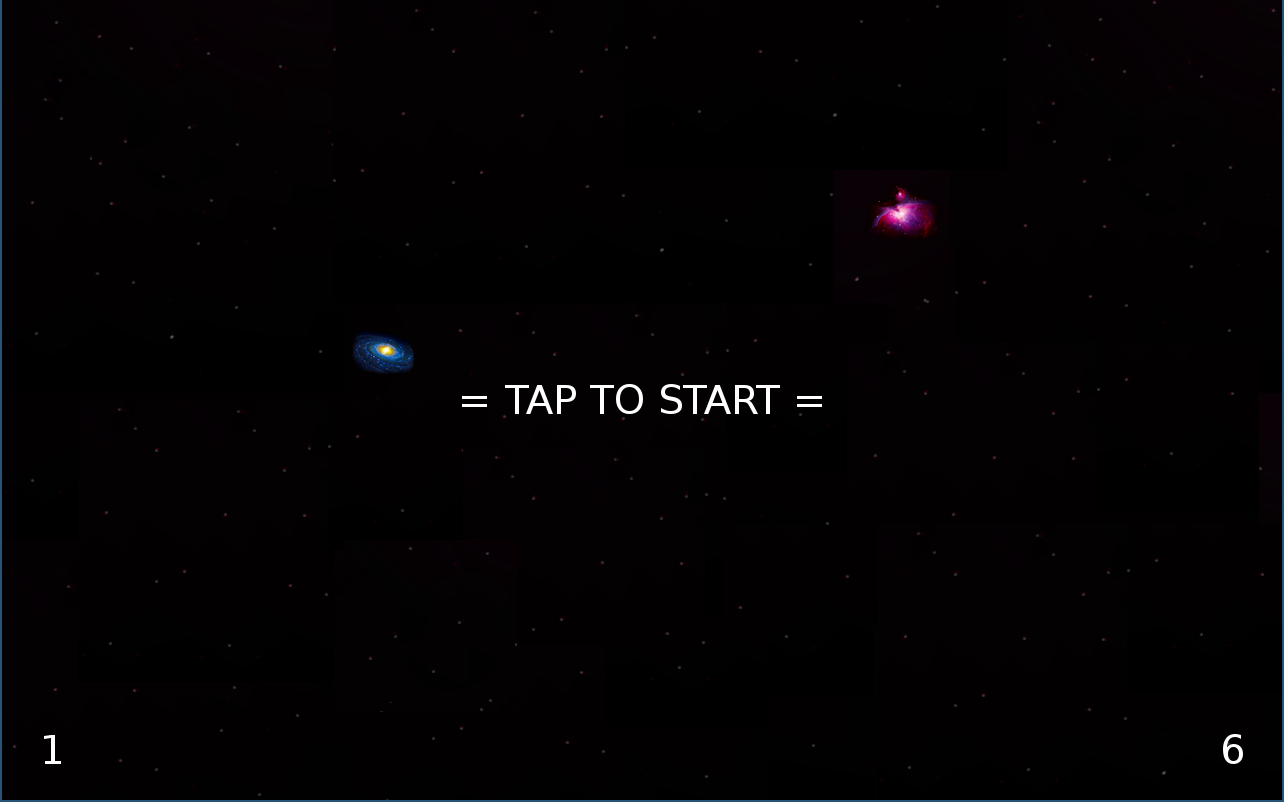
\includegraphics[scale=0.223]{screen-0.png}
\\
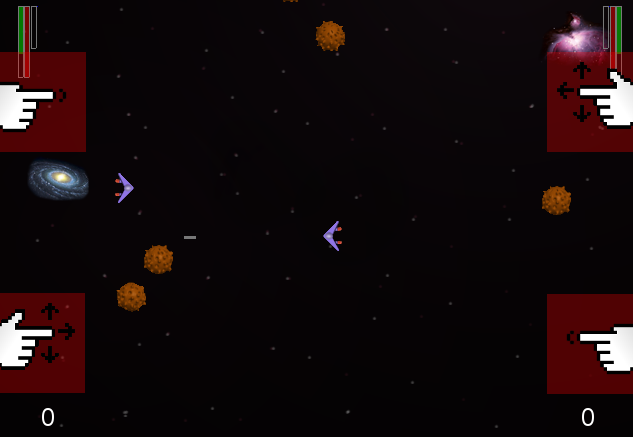
\includegraphics[scale=0.45]{screenshot.png}
\caption{
Screenshots for the game "Rocks!":
starting screen and gameplay with the player controls highlighted.
\label{fig.rocks}
}
\end{figure}

The "Rocks!" game of Figure~\ref{fig.rocks} is a spaceship shooter that two 
opponents play simultaneously on the same tablet.
Each player controls a spaceship by swiping and tapping different areas of the 
screen:
a swipe changes the ship acceleration to follow it;
a tap fires in the direction of the opponent.
At random periods, a new meteor enters the screen and moves to a random 
position.
If a ship collides with a meteor or an opponent shot, it explodes and the game 
restarts.
The scores on the bottom of the screen show the opponents' number of deaths.

\begin{figure}[t]
\begin{lstlisting}[numbers=left,xleftmargin=3em]
input void SDL_QUIT;
input int  SDL_DT;
input void SDL_REDRAW;
input _SDL_TouchFingerEvent* SDL_TOUCH;

interface IScore with
    var   _SDL_Point position;
    event void       go_increment;
end

interface IController with
    var   float ax, ay;
    event void  ok_shoot;
end

interface ICollidable with
    var   int       id;
    var   _SDL_Rect rect;
    event void      go_hit;
end

interface IShip with
    interface ICollidable;
    var   IController& controller;
    pool  Shots[3]     shots;
    event void         ok_destroyed;
end

#include "scores.ceu"
#include "controllers.ceu"
#include "collidables.ceu"
#include "ship.ceu"

par/or do
    await SDL_QUIT;
with
    every SDL_REDRAW do
        _SDL_RenderCopy(<bg-image>,<center>);
    end
with
    var Score score1 with
        this.position = <bottom-right>;
    end
    var Score score2 with
        this.position = <bottom-left>;
    end

    loop do
        do
            <...> // "TAP TO START" message
        end
        do
            <...> // gameplay with ships & meteors
        end
    end
with
    every SDL_REDRAW do
        _SDL_RenderPresent(<...>);
    end
end
\end{lstlisting}
%\rule{8.5cm}{0.37pt}
\caption{ File "main.ceu" with the top-level block of the game.
\label{lst.apps.rocks.1}
}
\end{figure}

The game is considerably more complex than the protocol of 
Section~\ref{sec.apps.srp}, so we generally describe the abstract interfaces 
and focus on the top-level block which puts all pieces together.
%
Figure~\ref{lst.apps.rocks.1} shows the relevant parts of the main file.
%
The game interacts with 4 input events (lines 1-4):
\code{SDL\_QUIT} requests the application to terminate (e.g., user closes the 
game window);
\code{SDL\_DT}, which is the source of all animations, is emitted on every 
frame passing the number of milliseconds elapsed since the previous frame;
\code{SDL\_REDRAW} requests screen updates and is also emitted on every frame;
\code{SDL\_TOUCH} signals screen touch events (i.e., tapping and swiping).
%
The interfaces (lines 6-27), with implementations included in corresponding 
files (lines 29-32), represent the abstract concepts that the main program 
manipulates:
\begin{description}
\item[\code{IScore}] (lines 6-9) represents the player scores, expecting a 
\code{position} in the screen (line 7), and exposing the event 
\code{go\_increment} which the application emits to increment the score (line 
8).
The actual implementation holds the score current state (e.g., points and 
graphical texture) and knows how to redraw itself on screen in reactions to 
\code{SDL\_REDRAW}.
\item[\code{IController}] (lines 11-14) represents the player controllers, 
exposing the current acceleration \code{ax}/\code{ay} charged to the ship (line 
12), and emitting \code{ok\_shoot}%
\footnote {
The prefixes \code{go\_} and \code{ok\_} for internal events informally 
represent direction: the application emits \code{go} events to interfaces, and 
awaits \code{ok} events emitted from them.
}
events which the application awaits to spawn new shots (line 13).
The actual implementation updates the acceleration according to reactions to 
the relevant \code{SDL\_TOUCH} inputs.
\item[\code{ICollidable}] (lines 16-20) represents all objects that require 
collision detection: the ships, shots, and meteors.
The field \code{id} (line 17) identifies the object when applying collisions 
(e.g., collisions between two meteors are ignored).
The field \code{rect} (line 18) exposes the current position and dimension for 
collision detection.
The application emits the \code{go\_hit} event to signal that the object has 
collided (line 19).
\item[\code{IShip}] (lines 22-27) represents the ships and extends the 
\code{ICollidable} interface (line 23).
A ship expects a \code{controller} reference (line 24) and holds a pool of 3 
shots (line 25, described further).
It also emits the event \code{ok\_destroyed} after dyeing (line 26).
\end{description}

The body of the game is a \code{par/or} (lines 34-60) that terminates on a
\code{SDL\_QUIT} request (line 35).
%
Reactions to \code{SDL\_REDRAW} relies on deterministic scheduling respecting 
the lexical order of trails: first, the trail in lines 37-39 redraws the 
background; then, all organisms inside the trail in lines 41-55 have the chance 
to redraw themselves (i.e., scores, ships, etc.); finally, the trail in lines 
57-59 updates the screen.

The core of the game resides in the trail in lines 41-55.
We first instantiate the scores as static organisms that survive the whole game 
(lines 41-46).
Then, we switch between the starting tap and gameplay behaviors of 
Figure~\ref{fig.rocks}, putting them in sequence and surrounded with loop 
(lines 48-55).
The \code{do-end} enclosing each behavior isolates one from another, i.e., no 
variables or organisms should survive when switching between them.

\begin{figure}%[t]
\begin{lstlisting}[numbers=left,xleftmargin=3em]
watching SDL_TOUCH do
    loop do
        await 500ms;        // message off
        watching 500ms do   // message on
            every SDL_REDRAW do
                _SDL_RenderCopy(<tap-msg>,<center>);
            end
        end
    end
end
\end{lstlisting}
%\rule{8.5cm}{0.37pt}
\caption{ The starting tap behavior in "main.ceu".
\label{lst.apps.rocks.2}
}
\end{figure}

The behavior for the starting tap, expanded in Figure~\ref{lst.apps.rocks.2}, 
is to blink the \emph{``TAP TO START''} message until the user taps the screen.
The \code{watching} composition terminates on the occurrence of 
\code{SDL\_TOUCH} (line 1), switching to the gameplay (lines 52-54 of 
Figure~\ref{lst.apps.rocks.1}).
In the meantime, the loop (lines 2-9) blinks the text on screen by alternating 
between an idle period of 500ms (line 3), and a displaying period of 500ms 
(lines 4-8).

\begin{figure}%[t]
\begin{lstlisting}[numbers=left,xleftmargin=3em]
var TouchController controller1 with
    this.move_region = <swipe-region-1>;
    this.fire_region = <tap-region-1>;
end
var TouchController controller2 with
    this.move_region = <swipe-region-2>;
    this.fire_region = <tap-region-2>;
end

var Ship ship1 with
    this.id         = SHIP1;
    this.rect       = <pos-dim-1>;
    this.controller = controller1;
end
var Ship ship2 with
    this.id         = SHIP2;
    this.rect       = <pos-dim-2>;
    this.controller = controller2;
end

pool Meteor[] meteors; // Meteor in collidables.ceu

par/or do
    every (1000 + _rand()%2000)ms do
        spawn Meteor in meteors;
    end
with
    every SDL_DT do
        loop (ICollidable*) c1 in <all> do
            loop (ICollidable*) c2 in <all> do
                if collides(c1,c2) and
                   enemies(c1,c2) then
                    emit c1:go_hit;
                    emit c2:go_hit;
                end
            end
        end
    end
with
    await ship1.ok_destroyed;
    emit points2.go_inc;
with
    await ship2.ok_destroyed;
    emit points1.go_inc;
end
\end{lstlisting}
%\rule{8.5cm}{0.37pt}
\caption{ The gameplay behavior in "main.ceu".
\label{lst.apps.rocks.3}
}
\end{figure}

The code for the gameplay is expanded in Figure~\ref{lst.apps.rocks.3}.
%
First, we declare the two controller organisms (lines 1-8), passing the move 
and fire regions in which they operate inside the screen (as illustrated in 
Figure~\ref{fig.rocks}).
After the declarations, each controller body reacts to \code{SDL\_TOUCH} swipe 
and tap events to either update its \code{ax} and \code{ay} fields, or emit 
\code{ok\_fired} events to the application, as specified by the 
\code{IController} interface.
%
Then, we declare the two ship organisms (lines 10-19), specifying the collision 
identifiers, starting position and dimensions, and controllers for each ship.
A ship knows how to move according to \code{SDL\_DT} frame events and its 
controller acceleration, as well as to redraw itself on screen on every 
\code{SDL\_REDRAW} request.
%
New meteors are spawned at most every 2 seconds (lines 24-26) and reside in a 
dedicated pool (line 21).
The meteors move to random positions and terminate themselves when leaving the 
screen, being automatically removed from the pool.
%
On every frame, we check for collision between all \code{ICollidable} organisms 
in the game, two by two, including all meteors, ships, and shots (lines 
28-38)%.
\footnote{
The real code (which is considerable more complex in this case) avoids 
comparing each pair twice and uses a temporary helper vector to hold all static 
and dynamic \code{ICollidables} in the same structure (illustrated by the 
\code{<all>} placeholder in lines 29-30).
}:
we compare their \code{rect} and \code{id} fields (inside \code{collides} and 
\code{enemies} calls in lines 31-32) and, if it is the case, we signal both
instances that they have collided (lines 33-34).
%
The gameplay terminates when either of the ships signal its destruction (line
40 or 43).
In this case, the program increments the enemy points (line 41 or 44) and 
aborts the whole \code{par/or}, switching back to the starting tap behavior.

Remind that a \code{do-end} encloses the gameplay behavior and isolates its 
state from the starting tap behavior (lines 52-54 of 
Figure~\ref{lst.apps.rocks.1}), making the controllers, ships, shots, and all 
meteors to go out of scope.
However, the \code{Score} organisms have a broader scope and persist for the 
whole game session (lines 41-46 of Figure~\ref{lst.apps.rocks.1}).

\begin{figure}%[t]
\begin{lstlisting}[numbers=left,xleftmargin=3em]
class Ship with
    <...>   // see IShip
do
    par/or do
        var int hits = 3;
        every this.go_hit do
            hits = hits - 1;
            if hits == 0 then
                break;
            end
        end
    with
        every this.controller.ok_fired do
            spawn Shot in this.shots with
                <...>   // direction, speed
            end
        end
    with
        var float vx = 0;
        var float vy = 0;
        var int dt;
        every dt in SDL_DT do
            vx = vx + this.controller.ax*dt;
            vy = vy + this.controller.ay*dt;
            this.rect.x = this.rect.x + vx*dt/1000;
            this.rect.y = this.rect.y + vy*dt/1000;
        end
    with
        every SDL_REDRAW do
            _SDL_RenderCopy(<image>,<pos>);
        end
    end
    emit ok_destroyed;
end
\end{lstlisting}
%\rule{8.5cm}{0.37pt}
\caption{ The \code{Ship} class in "ship.ceu".
\label{lst.apps.rocks.4}
}
\end{figure}

The code for the \code{Ship} class is presented in 
Figure~\ref{lst.apps.rocks.4}.
%
A ship has to be inflicted 3 hit points to be destroyed (lines 5-11).
Once this happens, the enclosing \code{par/or} terminates (lines 4-32) and 
emits the \code{ok\_destroyed} event to the application (line 33), which makes 
the gameplay to also terminate (lines 40-44 of Figure~\ref{lst.apps.rocks.3}).
%
Whenever the controller senses a tap and emits the \code{ok\_fired} event 
(lines 13-17), the ship spawns a new \code{Shot} organism in the direction of 
the opponent.
The pool of shots can only hold 3 simultaneous instances, meaning that further
\code{spawn} invocations fail until one of the shots leaves the screen (forcing 
the player to fire wisely).
%
For the ship movement (lines 19-27), we integrate its position with respect to 
the \code{dt} ``delta time'' acquired every frame, also taking into account the 
current controller acceleration.
%
Finally, we redraw the ship image in its current position for every 
\code{SDL\_REDRAW} request (lines 29-31).

\begin{figure}%[t]
\begin{lstlisting}[numbers=left,xleftmargin=3em]
class Missile with
    var Meteor* to_follow; // closest meteor
    <...>
do
    par/or do
        watching this.to_follow do
            every SDL_DT do
                if rect.y > to_follow:rect.y then
                    this.ay = -0.1;
                else
                    this.ay =  0.1;
                end
            end
        end
    with
        <...>   // missile moving, redrawing, etc
    end
end
\end{lstlisting}
%\rule{8.5cm}{0.37pt}
\caption{ The guided missile watches a pointer to a meteor.
\label{lst.apps.rocks.5}
}
\end{figure}

The complete game is below 500 lines of code and includes sound effects, 
explosions, power-up bonuses, guided missiles, indicative bars for hit points 
and available shots, among other features.
%
For the guided missiles, for instance, we use the \code{watching} construct to 
track the closest meteor that approaches the ship, as the code in 
Figure~\ref{lst.apps.rocks.5} shows.
The guided missile adjusts its acceleration on every frame (lines 7-13), based 
on the target position.
%
If the supervised meteor disappears (or is destroyed), the \code{watching} 
construct terminates (lines 6-14) and aborts the \code{par/or} (lines 5-17), 
making the guided missile to self-destruct.

\subsection{Discussion}

SSRP and \CEU rely on control compositions to express program flow concisely 
and in a structured way.
%
In contrast, solutions based on the observer pattern rely on explicit 
manipulation of global variables and state machines for flow control across 
reactions.
%
The presented applications express all control patterns exclusively with 
hierarchical compositions of activities and organisms, corroborating our 
previous experiments towards the eradication of state 
variables~\cite{ceu.sensys13},
%
In addition, control compositions enable the conception of new higher-level 
self-contained constructs, such as the syntactic sugars of 
Figure~\ref{fig.sugars} used in the applications.

Organisms are fundamental to expand SSRP to the development of more complex 
systems.
%
Organisms tie data and control together to form abstractions that can be 
deployed deliberately to a limited scope in applications.
%
In the protocol, the \code{Forwarder} and \code{Client} classes are defined in 
separate and applied to a restricted scope that does not mingle with the rest 
of the code.
%
Furthermore, the example uses anonymous (static and dynamic) instances that are 
completely autonomous and do not require explicit manipulation from the main 
program.
%
Finally, requests to stop the protocol trigger orthogonal abortion and 
finalization for all clients and forwarders, leaving the memory in a consistent 
state.
%
%We believe that such lexically scoped mechanism for modularity in applications 
%is a novel contribution of \CEU.

The distinction between static and dynamic organisms reflects more precisely 
the life cycle of each component in an application.
%
In the game, the two ships are declared static because they are alive during 
the whole scope of the gameplay; the meteors, in contrast, are declared dynamic 
because they terminate when disappearing from the screen, which is a runtime 
condition.
Nonetheless dynamic instances must still reside in static pools, also 
restricting them to a maximum lexical scope.
%
Even though this distinction exists in O.O. languages like C++, it does not 
apply effectively because the dependency in short-lived callbacks for reactive 
applications require all allocations to be dynamic in practice.

Static scopes helps developers to better understand the overall state of memory 
in applications: blocks in parallel coexist in memory; blocks in sequence do 
not; static organisms and pools coexist with their enclosing block.
%
This information is more difficult to infer when deallocation is explicit or 
relies on garbage collection, because both cases depend on runtime behavior 
that cannot be analyzed statically.
%
In the protocol, after a stop request, it is guaranteed that no forwarders or 
clients are in memory.
In the game, the memory for the starting screen and gameplay can never coexist 
because they are enclosed by blocks in sequence.

Explicit reference manipulation may introduce memory leaks even in garbage 
collected languages~\cite{dobbs.loiterers}.
For instance, a \emph{lapsed listener}~\cite{gamepatterns} is a pointer to an 
object---supposedly unreferred---that is not explicitly unregistered as a
listener from an event, preventing the garbage collector to release the object 
from memory.
%
When absolutely necessary, explicit manipulation in \CEU must be protected with 
the \code{watching} construct, which ensures that pointers to organisms do not 
hold them in memory.
%
In the game, the code for the guided missile that manipulates a reference to 
the closest meteor is automatically aborted when the latter goes out of scope.

% TODO:
%- points
    %- ship
    %- meteors

%- shots with [3]

\begin{comment}
interfaces, top-down development
also bottom up because each organism is independent

det scheduling -> reasoning -> also semantic tricks
\end{comment}

\section{Related work}
\label{sec.related}

%Even though Simula and Esterel are considerably old languages, their core 
%ideas that apply to \CEU have not evolved significantly, namely objects with 
%an execution body, compositions with orthogonal abortion, and the reactive 
%synchronous model.

\begin{comment}
Esterel provides module abstractions through the \code{run} command, which 
syntactically replaces the command by the referred module 
body~\cite{esterel.primer}.
%
Similarly, ESPranto~\cite{espranto} extends Esterel with a macro-based 
abstraction mechanism that enables the creation of domain specific languages.
%
However, macros expand at compile-time, being impossible to describe dynamic 
instantiation.
Furthermore, each use of a macro results in code replication, having a negative 
impact on code size.
\end{comment}

Simula is a simulation language that introduced the concepts of objects and 
coroutines~\cite{simula}.
%
The syntactic structure of classes in Simula is very similar to \CEU, exposing 
an interface that encapsulates an execution body.
%
However, the underlying execution models are fundamentally distinct:
\CEU employs a reactive scheduler to resume trails based on external stimuli, 
while Simula relies on cooperation (i.e., \code{detach} and \code{resume} 
calls, at the lowest level).
%
Simula has no notion of compositions, with each object having a single line of 
execution.
In particular, the lack of a \code{par/or} precludes orthogonal abortion and 
many derived \CEU features, such as lexically scoped organisms, finalization, 
and reference watching.
%
Without scopes, Simula objects have to live on the heap and rely on garbage 
collection.
%As far as we know, Simula processes cannot be terminated explicitly from other 
%processes.
%
%Finally, the conjunction of compositions with the synchronous model of \CEU 
%enables a XXX of static analysis, such as concurrent accesses to 
%variables~\cite{ceu.sensys13}.

Some previous work extend Esterel to provide dynamic synchronous 
abstractions~\cite{rp.scripts,rp.oo,sugarcubes}.
%
In particular, ReactiveML~\cite{rml} is a functional variant of Esterel with 
rich dynamic synchronous abstractions through \emph{processes}.
%Processes are functions that support hierarchical reactive constructs, such as 
%parallel compositions and an await primitive, similarly to organism bodies in 
%\CEU.
%A process can express dynamic instantiation with recursive invocations in 
%parallel with its own body.
%
However, these languages rely on heap allocation and/or garbage collection and 
may not be suitable for constrained embedded systems.
%
%\CEU programs, however, can use dynamic organisms that reside on static memory 
%(through bounded pools).
%
They also lack a finalization mechanism that hinders proper orthogonal abortion 
in the presence of stateful resources.
%For instance, \CEU relies on finalization for handling stateful resources as 
%well as for watching references.

Finally, the main distinction to existing work is how \CEU incorporates to SSRP 
the fundamental concept in SP of lexically scoped variables.
%
All constructs of \CEU have a clear and unambiguous lifespan that can be 
inferred statically from the source code.
%
Lexical scope permeates all aspects of the language:
Any piece of data or control structure has a well-defined scope that can be 
abstracted as an organism and safely aborted through finalization.
%
Even dynamic instances of organisms reside in scoped pools with the same 
properties.
%
%Assignments of organisms references with incompatible scopes are refused.

Functional Reactive Programming~\cite{frp.principles} contrasts with SSRP as a
complementary programming style for reactive applications.
%
We believe that FRP is more suitable for data-intensive applications, while 
SSRP, for control-intensive applications.
%
On the one hand, FRP uses declarative formulas to specify continuous functions 
over time, such as for physics or data constraints among entities, while SSRP 
requires explicit loops to update data dependencies continuously.
%
On the other hand, describing a sequence of steps in FRP requires to encode 
explicit state machines so that functions can switch behavior depending on the 
current state.

In the asynchronous spectrum of concurrency, a number of actor-based languages 
extend objects with independent execution contexts that communicate exclusively 
through message 
passing~\cite{agha.salsa,actors.thorn,actors.jcobox,actors.capsule}.
%
On the one hand, the inherent nondeterministic execution of actors demands full 
state isolation which makes distribution and many-core parallelism more 
straightforward.
%
On the other hand, the implicit synchronization in \CEU provides safe data 
sharing and global consensus about the overall state of the system, enabling 
abortion and lexical scopes for compositions.

\begin{comment}
- asynchronous langs
- Esterel + descendants
- CRP
- simula
- FRP

interactive  vs reactive
asynchronous vs synchronous
dataflow vs control
dynamic vs static

imperative
    - sequential (eliminates state machines)
    - better resource control
    - less abstract

dataflow

exemplo data melhor vs control melhor

The synchronous concurrency model...

We show composability, sequential, imperative
safety
Then, we extend synchronous reactive programming with dynamic

control vs data reactivity
\end{comment}

\section{Conclusion}
\label{sec.conclusion}

\begin{comment}
We believe that programming reactive systems can benefit from SSRP in \CEU:

\begin{itemize}
\item The synchronous model enables simpler reasoning about concurrency and is 
        fundamental to provide orthogonal abortion of activities.
\item With orthogonal abortion, an (unaltered) activity can be safely aborted 
        from other activities.
\item The finalization mechanism of \CEU extends orthogonal abortion for 
        activities that deal with stateful resources.
\item Static and dynamic organisms abstractions extend the domain of SSRP to a 
        wide range of applications and platforms.
\item Lexical scope for organisms provides seamless control of memory for SSRP, 
        eliminating memory leaks and the need for garbage collection.
\end{itemize}
\end{comment}

\CEU provides comprehensive support for structured synchronous reactive 
programming, extending classical structure programming with continuous 
interaction with the environment.

\CEU introduces organisms which reconcile data and control state in a single 
abstraction.
%
In contrast with objects, organisms have an execution body that can react 
independently to stimuli from the environment.
An organism body supports multiple lines of execution that can await events 
without loosing control context, offering an effective alternative to the 
infamous ``callback hell''.
%
Both static and dynamic instances of organisms are subject to lexical scope 
with automatic memory management, which eliminates memory leaks and the need 
for a garbage collector.

\CEU is suitable for wide range of reactive applications and platforms.
%
We have been experimenting with it in constrained platforms for sensor networks 
as well as in full-fledged computers and tablets for games and graphical 
applications%
\footnote{Uses of \CEU: \URL{http://www.ceu-lang.org/wiki/index.php?title=Uses}}.
%
%\CEU successfully participated in the \emph{Google Summer of Code}%
%\footnote{LabLua GSoC'14: 
%\small{\URL{http://google-opensource.blogspot.com/2014/08/google-summer-of-code-new-organizations.html}}}
%with a student that had no previous experience with the language.
%
We have also been teaching \CEU as an alternative language for sensor networks 
for the past two years in high-school and undergraduate levels.
%
Our experience shows that students take advantage of the sequential style of 
\CEU and can implement non-trivial reactive programs in a couple of weeks.

%care with embedded systems
%- pool
%- GC

%- examples w/o watching

%- games

%- wsn

\begin{comment}

===============================================================================

In computing, reactive programming is a programming paradigm oriented around data flows and the propagation of change. This means that it should be possible to express static or dynamic data flows with ease in the programming languages used, and that the underlying execution model will automatically propagate changes through the data flow.

For example, in an imperative programming setting, a := b + c would mean that a is being assigned the result of b + c in the instant the expression is evaluated. Later, the values of b and c can be changed with no effect on the value of a.

In reactive programming, the value of a would be automatically updated based on 
the new values.

===============================================================================

There seems to be a lot of confusion about Reactive Programming. What is it? Who created it?

The earliest reference I could find was written by Gérard Berry (one of the creators of the Esterel dataflow language) in his 1989 paper, “Real time programming: Special purpose or general purpose languages.” I emailed him to see if he knew of an earlier use. Mr. Berry pointed me to the 1985 paper, "On the development of reactive systems" by David Harel and Amir Pnueli. After contacting Professor Harel, he confirmed that they where the originators of the term.

So it would seem that Reactive Programming is at least 30 years old.

Harel and Pnueli’s paper discussed designing reactive systems in general, software or hardware. Their definition was…

    “Reactive systems… are repeatedly prompted by the outside world and their role is to continuously respond to external inputs.”

    D. Harel and A. Pnueli, “On the Development of Reactive Systems” (1985)

Mr. Berry’s paper focused on the software aspects of Reactive Programming

    “It is convenient to distinguish roughly between three kinds of computer programs. Transformational programs compute results from a given set of inputs; typical examples are compilers or numerical computation programs. Interactive programs interact at their own speed with users or with other programs; from a user point of view a time-sharing system is interactive. Reactive programs also maintain a continuous interaction with their environment, but at a speed which is determined by the environment, not by the program itself. Interactive programs work at their own pace and mostly deal with communications, while reactive programs only work in response to external demands and mostly deal with accurate interrupt handling.

    Real-time programs are usually reactive. However, there are reactive program that are not usually considered as being real-time, such as protocols, system drivers or man-machine interface handlers. All reactive programs require a common programming style.

    Complex applications usually require establishing cooperation between the three kinds of programs. For example, a programmer uses a man-machine interface involving menus, scroll bars and other reactive devices. The reactive interface permits him to tell the interactive operating systems to start transformational computations such as program compilations.”

    Berry, Gérard. “Real time programming: Special purpose or general purpose languages.” (1989)

From the preceding quotes we can say that reactive programs

    Activate in response to external demands
    Mostly deal with handling parallelism
    Operate at the rate of incoming data
    Often work in cooperation with transformational and interactive aspects

The definition of dataflow is a little more vague. Any system where the data moves between code units and triggers execution of the code could be called dataflow, that includes reactive systems. Thus, I consider Reactive Programming to be a subset of dataflow but a rather large subset. In casual use, Reactive Programming it is often a synonym for dataflow.

In more recent years Reactive Programming has become associated with two elements. Microsoft’s Reactive Extensions and Typesafe’s Reactive Manifesto.

Some people believe that Erik Meijer (formerly of Microsoft) and Jonas Bonér (of Typesafe) are trying to claim an old idea and call it their own. I am quite sure both of them are very aware of all of the previous work that has gone into Reactive Programming and dataflow. Mr. Bonér wrote about his observations on the resurgence of old techniques to solve new problems…

    “…Over the last few years we have seen quite a few different techniques and tools emerge in the industry as a way to address these new requirements. Some of them are old and proven, but to a large extent forgotten techniques, while others are novel and creative.”

    Why Do We Need a Reactive Manifesto

Reactive Programming and dataflow are old ideals that are being rediscovered because they help us solve problems we currently face.
\end{comment}

\begin{comment}
\section{A Reactive Concurrency Model}
\label{sec.models}

``Reactive systems'' are not a new class of software and have been first 
described by Harel as being ``repeatedly prompted by the outside world and 
their role is to continuously respond to external 
inputs''~\cite{statecharts.reactive}.
%
Berry goes further and makes a subtle distinction between ``interactive'' and 
``reactive'' systems~\cite{rp.synchronous}, in which the former communicate 
``at their own speed with users or with other programs'', while the latter, 
``at a speed which is determined by the environment, not by the program itself.
%
Overall, \emph{synchronous languages} deal with reactive systems better, while 
\emph{asynchronous languages}, with interactive systems~\cite{esterel.crp}.
%
Both authors propose synchronous languages for designing reactive systems 
(Statecharts~\cite{statecharts.visual} and Esterel~\cite{esterel.ieee91}).

%begin{comment}
In comparison to traditional ``transformational systems'', he recognizes 
reactive systems as ``particularly problematic when it comes to finding 
satisfactory methods for behavioral description''.
%
Berry goes further and makes a subtle distinction between ``interactive'' and 
``reactive'' systems~\cite{rp.synchronous}:
%
\begin{itemize}
\item Interactive programs interact at their own speed with users or with other 
programs; from a user point of view a time-sharing system is interactive.
\item Reactive programs also maintain a continuous interaction with their 
environment, but at a speed which is determined by the environment, not by the 
program itself.
\end{itemize}

%He states that ``interactive programs work at their own pace and mostly deal 
%with communications, while reactive programs only work in response to external 
%demands and mostly deal with accurate interrupt handling.''

This distinction is fundamental because the different control perspectives 
(i.e., ``at the speed of the program'' vs ``at the speed of the environment'') 
implies the use of different underlying concurrency models.
%end{comment}

The synchronous execution model is based on the hypothesis that internal 
computations (\emph{reactions}, in this context) run infinitely faster than the 
rate of events that trigger them~\cite{rp.hypothesis}.
In other words, the input and corresponded output are simultaneous, because 
reactions takes no time.
A reaction represents a logical instant in which the system as a whole reacts 
synchronously before going to the next instant.
%
During a reaction, the environment is invariant and does not interrupt it%
\footnote{
An actual implementation enqueues incoming input events to process them in the 
next iterations.
}.
ADVANTAGES: deterministic, etc.

The asynchronous execution model is more general and does not make assumptions 
about implicit synchronization.
Each activity%
\footnote{We use the term activity to generically refer to a language's unit of 
execution (e.g., \emph{thread}, \emph{actor}, \emph{process}, etc.).}
in the system is independent from one another and executes at its own pace.
%
For instance, an activity can perform time-consuming operations (e.g., 
compression, cryptography) without obstructing other activities.
%
Independence of activities also makes many-core parallelism straightforward.
%
However, in order to coordinate activities at specific points, the programmer 
has to use explicit synchronization primitives (e.g., mutual exclusion or 
message passing).
% ADA, thread-based concurrency, CSP

%%%%%%%%%%%%%%%%%%%%%%%%%%%%%%%%%%%%%%%%%%%%%%%%%%%%%%%%%%%%%%%%%%%%%%%%%%%%%%%

%begin{comment}
\begin{figure}
\centering
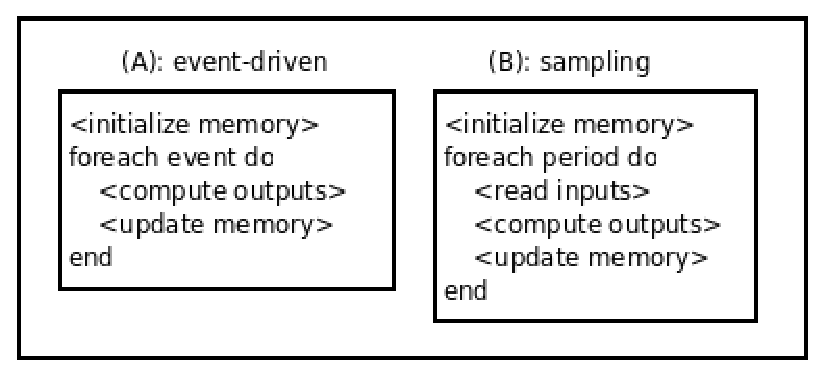
\includegraphics[width=3.0in]{sync_impl.eps}
\caption{Schedulers for synchronous systems}
\label{fig.impl}
\end{figure}
% Esterel, HW, \CEU, observers

Figure \ref{fig.impl} shows two common implementation schemes for synchronous 
schedulers~\cite{rp.twelve}.
%
in the event-driven scheme, a loop iteration computes outputs for each event 
occurrence;
%
in the sampling scheme, a loop iteration computes the inputs and outputs on 
every clock tick.
%
In both cases, each loop iteration represents a logical instant in which the 
system as a whole reacts synchronously before going to the next instant.
%
During a reaction, the environment is invariant and does not affect the running 
iteration%
\footnote{
An actual implementation enqueues incoming input events to process them in the 
next iterations.
}.
%
Both schemes are compliant with the synchronous hypothesis, in which input and 
resulting output happen at the same time, considering this notion of time as a 
sequence of discrete events or clock ticks.
%end{comment}

%begin{comment}
%
Having the language to deal automatically with these features strengthen 
structured programming, because we can compose activities together.
%
For instance, although adding a new activity implies extra computational 
overhead, it does not affect the behavior of the other activities, which still 
depend only on the input timeline.
%
Furthermore, if we want to abort an existing activity given a new requirement, 
we can do it externally, without changing

 determinism and abortion with these issues is interesting allows to
compose activities while keeping them decoupled, because they need not to be 
NOtweaked to accommodate these requirements.


decoupling =>
structured programming

deterministic,
    reproducible
abortion
    structured programming
    no coupling
    just like

The way each side is implemented does not affect the behavior,
only the way you compose them (which is external to each implementation)

%
DET and ABRT
both yield to better reasoning
behave the same with or without concurrency
%end{comment}

%%%%%%%%%%%%%%%%%%%%%%%%%%%%%%%%%%%%%%%%%%%%%%%%%%%%%%%%%%%%%%%%%%%%%%%%%%%%%%%

\subsection{Deterministic execution}

In the context of reactive applications, we interpret determinism as 
reproducible execution given the same sequence of stimuli, i.e., the outcome 
depends exclusively of an external input timeline, in contrast with internal 
scheduling and communication timings.

Figure~\ref{lst.leds} shows three implementations for an application that 
blinks two LEDs in parallel with different frequencies.
We use two asynchronous languages (a CSP-based~\cite{arduino.occam} and a 
thread-based~\cite{arduino.chibios} language), and also the synchronous 
language \CEU.
%
The intent and syntactic structure of the implementations are similar:
composing the two blinking activities in parallel.
%
The LEDs should blink together every 3 seconds (the least common denominator 
between 600ms and 1s).
%
As we expected, the LEDs in the two asynchronous implementations loose 
synchronism after some time of execution, while the implementation in \CEU 
remains synchronized forever.

The example highlights how the inherent non-determinism in the asynchronous 
model makes hard to (blindly) compose activities supposedly synchronized: 
unpredictable scheduling as wall as latency in message-passing eventually cause 
observable asynchronism.
%
In \CEU, the \code{await} is the only primitive that takes time, but which the 
programmer uses explicitly to conform with the problem specification.
The language runtime compensates the internal timings for communication and 
computation (which the programmer cannot control) to conform with the model and 
remain synchronized~\cite{ceu.sensys13}.
%
Arguably, reasoning over \code{await} statements is simpler than also having to 
consider all other statements of the language.

\begin{figure}%[t]
\begin{minipage}[t]{0.34\linewidth}
\begin{lstlisting}
// OCCAM-PI
PROC main ()
 CHAN SIGNAL s1,s2:
 PAR
  PAR
   tick(600, s1!)
   toggle(11, s1?)
  PAR
   tick(1000, s2!)
   toggle(12, s2?)
:

\end{lstlisting}
\end{minipage}
%
\begin{minipage}[t]{0.33\linewidth}
\begin{lstlisting}
// ChibiOS
void thread1 () {
  while (1) {
    sleep(600);
    toggle(11);
  }
}
void thread2 () {
  while (1) {
    sleep(1000);
    toggle(12);
  }
}
void setup () {
  create(thread1);
  create(thread2);
}

\end{lstlisting}
\end{minipage}
%
\begin{minipage}[t]{0.31\linewidth}
\begin{lstlisting}
// Ceu
par do
  loop do
    await 600ms;
    _toggle(11);
  end
with
  loop do
    await 1s;
    _toggle(12);
  end
end
\end{lstlisting}
\end{minipage}
%
%\rule{8.5cm}{0.37pt}
\caption{ Two blinking LEDs in OCCAM-PI, ChibiOS and \CEU.\newline
{\small %\textmd{
%The lines of execution in parallel blink two LEDs (connected to ports 11 and 
%12) with different frequencies.
%Every 3 seconds the LEDs should light on together.
}%}
\label{lst.leds}
}
\end{figure}

%%%%%%%%%%%%%%%%%%%%%%%%%%%%%%%%%%%%%%%%%%%%%%%%%%%%%%%%%%%%%%%%%%%%%%%%%%%%%%%

\subsection{Orthogonal abortion}

%begin{comment}

On the other hand, the synchronous hypothesis does not hold for reactions that 
have latency (e.g., network communication or algorithm-intensive computations),
however, does not apply when the computation involves latency:
problem communication takes time
either communication or time consuming operations
because now, at the speed of the program

parallelism
latency

For reactive systems zzz
For highly synchronous systems, the sole synchronization overhead, which is 
non-existent in XXX, may neutralize any gains with parallelism.
% or even worsen parallelism

Illustrate with two examples:
that explore the advantages of synchronous:
reasoning in concurrency
seamless composition

communitacions is directed and takes time (because the receiver may not be 
waiting)

The synchronous model
input => output
broadcast possible
global consensus possible
determinism
simpler model

In synchronous systems, communication is instantaneous.
The zero-delay property of the synchronous hypothesis guarantees that no time 
elapses between event announcement and receiving.
Also, as communication is via broadcast, all systems parts share the same 
information all the time.
These two characteristics make global data consensus another property of 
synchronous systems.

conclusion:
no blind/free/orthogonal composition
no deterministic/reproducible execution
parallelism / no-forced synch
time-consuming / independent

A recent Reactive Manifesto

synchronous reactive
vs
asynchronous reactive

Even tough the presented deterministic and abortion examples can be properly 
implemented in asynchronous languages, they require to tweak the activities 
with mutual
synchronization primitives.
%
This increases the coupling degree among activities with concerns that are not 
directly related to the problem specification.

The two models suggest a tradeoff between unrestricted execution with real 
parallelism versus structural composability with deterministic behavior.
%
For reactive applications with continuous and real-time concurrency, we believe 
that the synchronous execution model is more appropriate.

\end{comment}

\bibliographystyle{abbrv}
\bibliography{other,my}

\end{document}
